\documentclass[a4paper,12pt]{article}
% This file was converted to LaTeX by Writer2LaTeX ver. 0.4
% see http://www.hj-gym.dk/~hj/writer2latex for more info
\usepackage[ascii]{inputenc}
\usepackage[T1]{fontenc}
\usepackage[english,portuges]{babel}
\usepackage{amsmath,amssymb,amsfonts,textcomp}
\usepackage{color}
\usepackage{calc}
\usepackage{hyperref}
\hypersetup{colorlinks=true, linkcolor=blue, filecolor=blue, pagecolor=blue, urlcolor=blue}
\usepackage{graphicx}
\newcommand\textsubscript[1]{\ensuremath{{}_{\text{#1}}}}
% Pages styles (master pages)
\makeatletter
\newcommand\ps@Standard{%
\renewcommand\@oddhead{}%
\renewcommand\@evenhead{}%
\renewcommand\@oddfoot{}%
\renewcommand\@evenfoot{}%
\setlength\paperwidth{21.001cm}\setlength\paperheight{29.7cm}\setlength\voffset{-1in}\setlength\hoffset{-1in}\setlength\topmargin{3cm}\setlength\headheight{12pt}\setlength\headsep{0cm}\setlength\footskip{12pt+0cm}\setlength\textheight{29.7cm-3cm-2.499cm-0cm-12pt-0cm-12pt}\setlength\oddsidemargin{2.499cm}\setlength\evensidemargin{2.499cm}\setlength\textwidth{21.001cm-2.499cm-2.499cm}
\renewcommand\thepage{\arabic{page}}
\setlength{\skip\footins}{0.101cm}\renewcommand\footnoterule{\vspace*{-0.018cm}\noindent\textcolor{black}{\rule{0.25\columnwidth}{0.018cm}}\vspace*{0.101cm}}
}
\makeatother
\pagestyle{Standard}
\everymath{\displaystyle}
\begin{document}
\clearpage\pagestyle{Standard}
{\centering\selectlanguage{english}\bfseries
SIMULA\c{C}\~AO NUM\'ERICA DE SISTEMAS DIN\^AMICOS
\par}


\bigskip

{\centering\selectlanguage{english}\bfseries
Guilherme de Azevedo Silveira
\par}

{\centering\selectlanguage{portuges}
Instituto de Matem\'atica e Estat\'istica {--} Universidade de S\~ao
Paulo\newline
R. do Mat\~ao, 1010 {--} Cidade Universit\'aria {--} CEP 05508{}-090
{--} S\~ao Paulo
\par}

{\centering\selectlanguage{english}
\href{mailto:gas@linux.ime.usp.br}{gas@linux.ime.usp.br}
\par}

{\centering\selectlanguage{english}\bfseries
Eduardo Colli
\par}

{\centering\selectlanguage{portuges}
Instituto de Matem\'atica e Estat\'istica {--} Universidade de S\~ao
Paulo\newline
R. do Mat\~ao, 1010 {--} Cidade Universit\'aria {--} CEP 05508{}-090
{--} S\~ao Paulo
\par}

{\centering\selectlanguage{portuges}
\href{mailto:colli@ime.usp.br}{\foreignlanguage{english}{colli@ime.usp.br}}
\par}


\bigskip

{\selectlanguage{english}\itshape
\textbf{Abstract. }\textmd{Este artigo descreve o processo de
idealiza\c{c}\~ao e realiza\c{c}\~ao de um software para uso de alunos
na \'area de matem\'atica aplicada com \^enfase em sistemas iterados.
Tamb\'em ser\'a tratada a id\'eia de ajudar pesquisas que estudam
bacias de atra\c{c}\~ao. O mais importante \'e que o estudante de
matem\'atica, professor ou pesquisador n\~ao deve ser obrigado a
aprender detalhes de uma linguagem de programa\c{c}\~ao para executar
simula\c{c}\~oes num\'ericas cl\'assicas podendo, ent\~ao, focar em
suas habilidades matem\'aticas. dynamical systems, java and
mathematics, numerical simulations.}}

{\selectlanguage{english}\itshape
\textbf{Abstract. }This paper describes the process of brainstorming,
developing and using an open source software in order to help
mathematics students dealing with iterated systems. It also aims at
helping researchs which are based on watching those
system{\textquotesingle}s iterations and attractors basins, giving the
feeling of what is going on. The main idea is that the math student,
teacher or researcher should not need to learn advanced topics of a
programming language in order to make some numeric simulations, so he
can focus on his mathematical analysis and skills. sistemas
din\^amicos, java e matem\'atica, simula\c{c}\~ao num\'erica.}

{\selectlanguage{english}\bfseries
1. A necessidade de uma ferramenta}

{\selectlanguage{english}
A medida que crescemos e aprendemos matem\'atica na escola ficamos cada
vez mais encantados com a m\'agica de analisar equa\c{c}\~oes complexas
e de vivenciar as mais belas propriedades num\'ericas. Tudo isso muda
uma vez que nos tornamos intelectualmente mais adultos e entramos na
faculdade, onde encontramos algumas dificuldades.}

{\selectlanguage{english}
 A maior parte dos alunos n\~ao lida t\~ao bem com programa\c{c}\~ao,
ferramenta que j\'a se provou extramente \'util em diversas \'areas da
matem\'atica aplicada. Mais grave ainda, isso n\~ao acontece somente
com alunos mas tamb\'em com diversos professores e pesquisadores que
t\^em o mesmo medo de programar.}

{\selectlanguage{english}
 A sala de aula seria um ambiente mais descontra\'ido e vivo se os
alunos fossem capazes de focar em suas t\'ecnicas matem\'aticas em vez
de ter que aprender os detalhes de shift de bits em C ou qualquer outra
linguagem de programa\c{c}\~ao: n\~ao importa se na pesquisa ou na
aula, muitas vezes o foco principal \'e na parte matem\'atica mas os
alunos e professores precisam gastar muito tempo extra para aprender
uma linguagem que talvez n\~ao seja o foco do mesmo naquele momento.}

{\selectlanguage{english}
 Dessas complica\c{c}\~oes nasce a necessidade de uma ferramenta que
torne opcional o conhecimento aprofundado de alguma linguagem de
programa\c{c}\~ao, sendo que ela ainda seria capaz de simular alguns
sistemas durante a aula, deixando a mesma mais interessante e os
exemplos mais pr\'aticos, possivelmente diminuindo o n\'umero de alunos
que dormem na aula.}

{\selectlanguage{english}
 O Iterador (Pulga) \'e um projeto escrito em Java e desenvolvido com o
foco em tornar poss\'ivel tudo isso que fora mencionado at\'e esse
instante.}

{\selectlanguage{english}\bfseries
2. Simula\c{c}\~ao de sistemas din\^amicos}

{\selectlanguage{english}\mdseries
2.1. O problema}

{\selectlanguage{english}
Um exemplo pr\'atico de uso desse software escrito em Java \'e a
simula\c{c}\~ao num\'erica de sistemas din\^amicos cont\'inuos ou
discretos atrav\'es de resultados gr\'aficos.}

{\selectlanguage{english}
 Um estudante que deseja ver o que acontece para determinada
condi\c{c}\~ao inicial do sistema com determinados par\^ametros pode
faz\^e{}-lo facilmente sem se preocupar com detalhes de como um
gr\'afico deve ser mostrado em uma tela como por exemplo t\'ecnicas de
double buffering etc.}

{\selectlanguage{english}
 Outro exemplo \'e o professor enriquecer uma aula mostrando para alunos
n\~ao somente na lousa os resultados n\'umericos de uma itera\c{c}\~ao
mas tamb\'em graficamente a \'orbita percorrida, facilitando aos alunos
{\textquotedbl}digerir{\textquotedbl} tudo aquilo que fora explicado na
aula.}

{\selectlanguage{english}\mdseries
2.2. A solu\c{c}\~ao}

{\selectlanguage{english}
Com a simples entrada da f\'ormula de itera\c{c}\~ao e a escolha do
espa\c{c}o a ser plotado na tela podemos simular a itera\c{c}\~ao de um
sistema.}

{\selectlanguage{english}
 Por exemplo, come\c{c}amos com o atrator de H\'enon (com a = 1.4 e b =
0.3) e configurando x1 para \textbf{1 {--} 1.4 * x1 * x1 {--} 0.3 * x2}
e x2 para \textbf{x1}\textmd{. Escolhendo o espa\c{c}o
\ }\textbf{{}-1.5 {\textless} x1 {\textless} 1.5 }\textmd{e
}\textbf{{}-1.5 {\textless} x2 {\textless} 1.5 }\textmd{temos o
resultado da esquerda da Figura 1.}}

{\centering\selectlanguage{english}\sffamily\bfseries
Figura 1. Attrator de Henon (a = 1.4, b = 0.3)
\par}

\begin{center}
 [Warning: Image ignored] % Unhandled or unsupported graphics:
%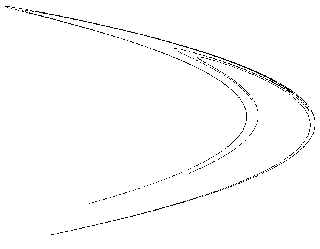
\includegraphics[width=5.95cm,height=4.5cm]{ime-img1.png}

\end{center}
{\selectlanguage{english}\mdseries
 Portanto o \'unico conhecimento que se faz necess\'ario \'e o de saber
a equa\c{c}\~ao do mapa. Uma vez que o programa compila todas as
equa\c{c}\~oes em c\'odigo Java, ele permite que o usu\'ario
avan\c{c}ado aprenda a linguagem e evolua para sistemas mais
complexos.}

{\selectlanguage{english}
 Resumindo, existem dois caminhos: usar os recursos b\'asicos simulando
itera\c{c}\~oes sem precisar conhecer conhecer uma linguagem ou se
aprofundar e obter resultados avan\c{c}ados.}

{\selectlanguage{english}\bfseries
3. Diagramas de bifurca\c{c}\~ao}

{\selectlanguage{english}
 \'E poss\'ivel simular um diagrama de bifurca\c{c}\~ao utilizando uma
funcionalidade bem simples do Iterador: basta configurar o tamanho do
intervalo ap\'os o qual a condi\c{c}\~ao inicial e os par\^ametros
devem ser alterados.}

{\selectlanguage{english}
 Por exemplo, supondo a exist\^encia de um par\^ametro \textbf{a} e
\textbf{x} sendo o espa\c{c}o de configura\c{c}\~ao: ap\'os o n\'umero
desejado de itera\c{c}\~oes para um determinado valor de \textbf{a
}esse \'ultimo deve ser incrementado e \textbf{x }\textmd{deve voltar
ao valor inicial para ir a pr\'oxima coluna e continuar com o diagrama,
sem nenhuma complexidade extra}:}

{\selectlanguage{english}
 a = a + 0.1;}

{\selectlanguage{english}
 x = x\_inicial;}

{\selectlanguage{english}
 Um exemplo pr\'atico \'e a fam\'ilia unidimensional cuja seq\"u\^encia
de iterados apresenta comportamento semelhante ao da seq\"u\^encia de
intervalos entre bolhas, quando uma mangueira de ar \'e injetada na
base de um l\'iq\"uido viscoso. O par\^ametro
{\textquotedbl}horizontal{\textquotedbl} (fi) corresponde \`a
mudan\c{c}a da vaz\~ao do ar. Mudar os valores de l corresponde a mudar
o comprimento da mangueira que injeta o ar (por incr\'ivel que
pare\c{c}a esse par\^ametro afeta bastante o resultado).\newline
 No c\'alculo de x\textmd{\textsubscript{k+1}} em fun\c{c}\~ao de
x\textsubscript{k} aparece uma fun\c{c}\~ao c\'ubica que depende deste
\'ultimo. \'E necess\'ario calcular a maior raiz desta fun\c{c}\~ao
portanto for a criada uma express\~ao intermedi\'aria (t0) que serve
para escolher uma condi\c{c}\~ao inicial para o m\'etodo de Newton, e a
outra (raiz) acha a ra\'iz propriamente dita iterando algumas vezes
esse m\'etodo.}

{\selectlanguage{english}
 A seguir, o exemplo do m\'etodo newton feito de maneira program\'atica
e ao lado esquerdo da figura 3 encontra{}-se o resultado desse
diagrama.}

{\selectlanguage{english}
 raiz = t0;}

{\selectlanguage{english}
 for (int i = 0; i {\textless} 20; i++)}

{\selectlanguage{english}
  \ \ \ \ raiz = (2*m*raiz*raiz*raiz {}- x1)/(3*m*raiz*raiz {--} l);}

{\selectlanguage{english}\bfseries
4. Plugins e flexibilidade}

{\selectlanguage{english}
A arquitetura que foi montada devido a id\'eia de utilizar Reflection
permite que diversas extens\~oes possam ser adicionadas ao programa.}

{\selectlanguage{english}
 Por exemplo, um professor pode criar um plugin onde fosse poss\'ivel
configurar padr\~oes de exporta\c{c}\~ao e disponibilizasse tais
plugins para os alunos que, por sua vez, ficam com duas op\c{c}\~oes:
escrever o c\'odigo java eles mesmos ou utilizar algo que o professor
criou.}

{\selectlanguage{english}
 O programa tamb\'em pode ser usado de certas maneiras que n\~ao foram
pensadas anteriormente pelos autores, ainda assim sem ter de programar.
Por exemplo, \'e poss\'ivel desenhar um conjunto de Mandelbrot, onde um
espa\c{c}o de par\^ametros \'e explorado para uma condi\c{c}\~ao
inicial fixa e pintado de acordo com sua \'orbita.}

{\selectlanguage{english}
 Um plugin simples que facilita o uso do programa \'e o de
condi\c{c}\~ao inicial, que permite selecionar diversos pontos que
ser\~ao utilizados para analisar suas \'orbitas em uma \'unica imagem.
No lado direito da Figura 2 podemos ver o resultado desse plugin para
diversas condi\c{c}\~oes iniciais em um mapa Ragazzo{}-Zanata:}

{\centering\selectlanguage{english}\mdseries
Figura 2. Diagrama de bifurca\c{c}\~ao do sistema das bolhas e
Ragazzo{}-Zanata
\par}

\begin{center}
 [Warning: Image ignored] % Unhandled or unsupported graphics:
%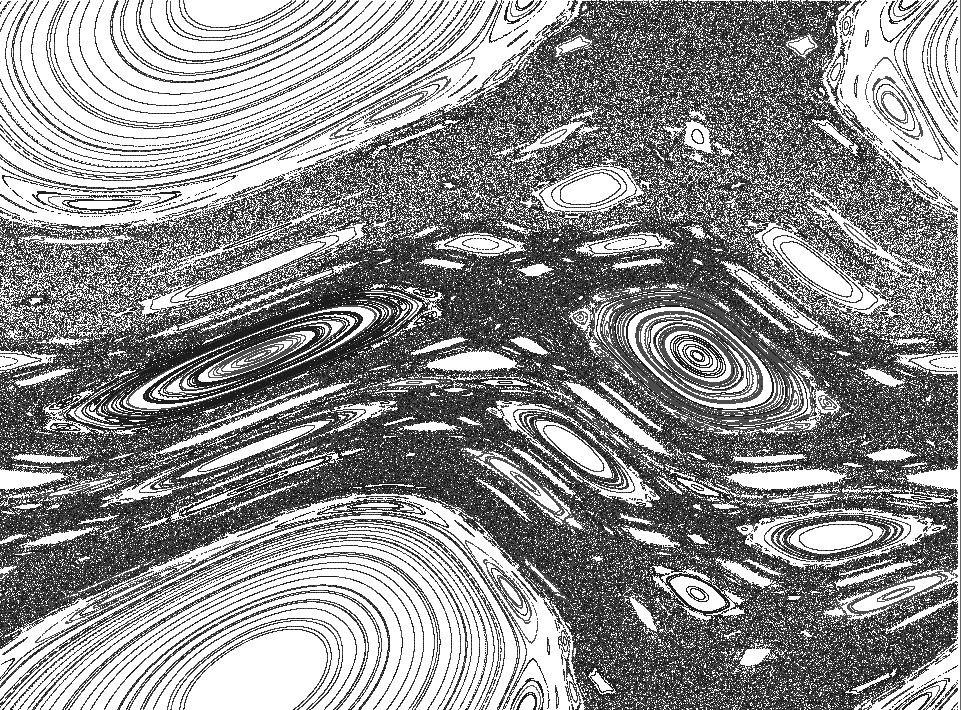
\includegraphics[width=5.42cm,height=4.001cm]{ime-img2.png}

\end{center}
\begin{center}
 [Warning: Image ignored] % Unhandled or unsupported graphics:
%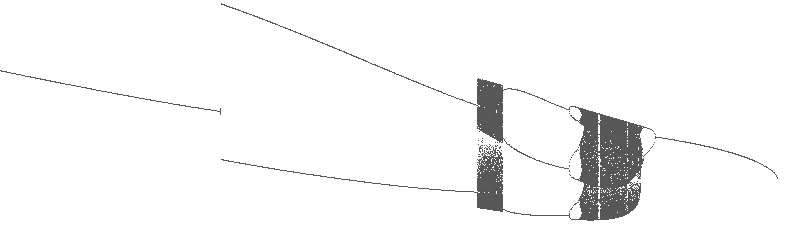
\includegraphics[width=10.4cm,height=4.001cm]{ime-img3.png}

\end{center}
{\selectlanguage{english}\bfseries
5. Bacia de atra\c{c}\~ao}

{\selectlanguage{english}\mdseries
5.1. O problema}

{\selectlanguage{english}
Diversas quest\~oes podem surgir sobre um sistema: como um conjunto de
pontos reage ap\'os n itera\c{c}\~oes? Para qual atrator a \'orbita de
determinados pontos converge? Ser\'a que \'e uma \'orbita peri\'odica?
Quantos atratores existem? Como lidar com o infinito? Um simples
processo de itera\c{c}\~ao n\~ao resolve tais perguntas.}

{\selectlanguage{english}\mdseries
5.2. A solu\c{c}\~ao}

{\selectlanguage{english}
 Com o plugin de bacia de atra\c{c}\~ao, o usu\'ario come\c{c}a
configurando o sistema como de costume. Em um segundo passo \'e
iniciado o Average Picker, que escolhe aleatoriamente pontos iniciais
contidos no espa\c{c}o definido e itera por eles. Usando um par de
fun\c{c}\~oes customiz\'aveis, ele calcula m\'edias dos pontos que
comp\~oe a \'orbita do ponto inicial.}

{\selectlanguage{english}
 Os resultados dessas m\'edias \'e mostrado em um canvas que representa
o espa\c{c}o das m\'edias, que tamb\'em \'e configur\'avel (inclusive
durante o processo!). A partir desse momento o usu\'ario pode
selecionar, atrav\'es de pol\'igonos, \'areas que chamamos de clouds e
identificam diferentes atratores marcados com cores \'unicas.}

{\selectlanguage{english}
 Se a itera\c{c}\~ao de um ponto inicial tem como resultado uma m\'edia
dentro de uma cloud, o programa conclu\'i que tal \'orbita foi
capturada pelo atrator e pinta esse ponto com a cor
pr\'e{}-determinada. Um pol\'igono que contem todos os outros pode ser
desenhado e define um \ ``atrator no infinito''.}

{\selectlanguage{english}\mdseries
5.3. Exemplo pr\'atico}

{\selectlanguage{english}
O programa foi testado com o mapa de H\'enon, par\^ametros a = 1.2, b =
0.2 e executando duas itera\c{c}\~oes por vez para simular dois
atratores. Configurando duas fun\c{c}\~oes de m\'edia, o sistema
desenha a bacia de atra\c{c}\~ao, ajudando ao aluno identificar quais
condi\c{c}\~oes iniciais convergem para quais atratores.}

{\selectlanguage{english}
  $\mathit{Media}_{1}=\sum {(\left|{x_{1}}\right|\ast
\left|{x_{2}}\right|)}$ (c\'odigo: Math.abs(x1) * Math.abs(x2))}

{\selectlanguage{english}
  $\mathit{Media}_{2}=\sum {(x_{1}\ast x_{1}+x_{2}\ast x_{2})}$
(c\'odigo: x1 * x1 + x2 * x2)}

{\selectlanguage{english}
 A Figura 3 mostra o resultado das m\'edias, o desenho de H\'enon nesse
caso e a bacia para a = 1.2 e b = 0.2 quando definidas tr\^es cores:
cinza escuro para uma nuvem, cinza claro para a outra, branco para o
infinito e preto para algo desconhecido.}

{\selectlanguage{english}
 Sendo assim, o pr\'oprio programa acaba incentivando o aluno a
descobrir o que s\~ao esses pontos pretos e para onde v\~ao as
\'orbitas dos mesmos.}

\begin{center}
 [Warning: Image ignored] % Unhandled or unsupported graphics:
%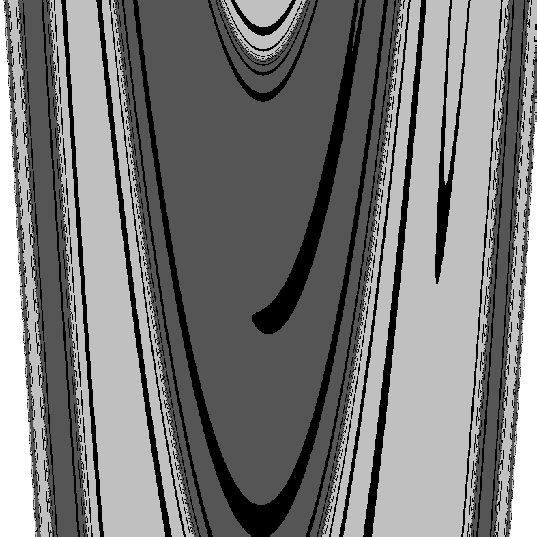
\includegraphics[width=4.5cm,height=4.5cm]{ime-img4.png}

\end{center}
\begin{center}
 [Warning: Image ignored] % Unhandled or unsupported graphics:
%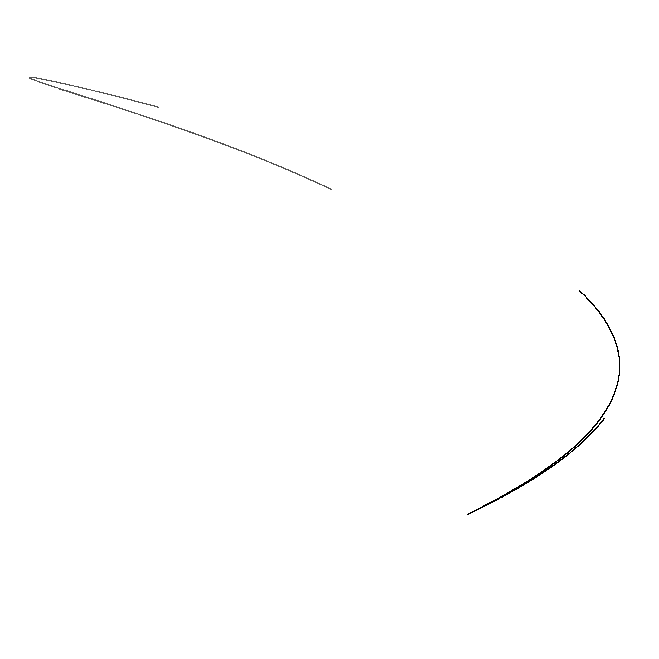
\includegraphics[width=4.731cm,height=4.5cm]{ime-img5.png}

\end{center}
{\centering\selectlanguage{english}\sffamily\bfseries
\textrm{\textmd{Figura 3. M\'edias de dois atratores, os atratores e a
bacia (H\'enon, a=1.2, b=0.2)}}
\par}

\begin{center}
 [Warning: Image ignored] % Unhandled or unsupported graphics:
%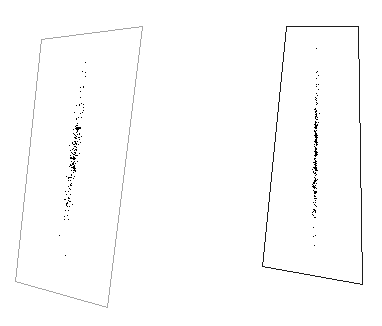
\includegraphics[width=5.339cm,height=4.5cm]{ime-img6.png}

\end{center}
{\selectlanguage{english}\bfseries
6. Tecnologias e padr\~oes utilizados}

{\selectlanguage{english}
Diversas tecnologias e padr\~oes s\~ao utilizados para garantir a
flexibilidade necess\'aria por esse software.}

{\selectlanguage{english}
 A primeira id\'eia foi de utilizar Java devido a natureza deste
programa: existe uma necessidade de executar um peda\c{c}o de c\'odigo
milh\~oes de vezes e o just{}-in{}-time compiler das m\'aquinas
virtuais (VM) que suportam a linguagem e tecnologia Java otimizam esse
c\'odigo.}

{\selectlanguage{english}
 J\'a os arquivos s\~ao salvos em formato xml atrav\'es de uma
biblioteca chamada Xstream, capaz de transformar objetos em c\'odigo
xml atrav\'es de um simples mapeamento de classes para tags e, em
conjunto com Reflection \'e poss\'ivel armazenar nesses arquivos
informa\c{c}\~oes sobre a pr\'opria estrutura das classes que estavam
sendo utilizadas como plugins ativos no momento de salvar o arquivo
etc.}

{\selectlanguage{english}
 Ainda baseado em Reflection mas j\'a com uma itera\c{c}\~ao maior com
Beanshell foi criada uma estrutura extremamente din\^amica de controle
de l\'ogicas simples para os menus do sistema e com o uso da primeira
tornou{}-se poss\'ivel gerar diversas janelas atrav\'es de arquivos de
configura\c{c}\~ao simples uma vez que a maior parte das tecnologias
dispon\'iveis para criar janelas (como thinlet por exemplo) foram
feitas para grandes sistemas comerciais, que n\~ao \'e exatamente o
tipo de software que fora desenvolvido.}

{\selectlanguage{english}
 Por fim, o Janino \'e a biblioteca utilizada para compilar as
express\~oes escritas pelo usu\'ario, dando suporte a diversas
estruturas da linguagem Java em sua vers\~ao 1.4. Classes s\~ao criadas
em tempo de execu\c{c}\~ao e embutidas no sistema atrav\'es de
classloaders tamb\'em gerados din\^amicamente pelo Janino que ent\~ao
passam a ser otimizados pela VM como explicado anteriormente, tirando
proveito de todas as otimiza\c{c}\~oes poss\'iveis em tempo de
execu\c{c}\~ao: a grande vantagem de n\~ao compilar nosso c\'odigo
estaticamente e usar uma linguagem din\^amica.}

{\selectlanguage{english}
 Outras id\'eia interessante para o usu\'ario final \'e a do Big Fat Jar
que permite criar um \'unico arquivo .jar que \'e o \'unico arquivo
necess\'ario para a execu\c{c}\~ao do programa fazendo com que o
usu\'ario leigo na computa\c{c}\~ao n\~ao sofra com as
complica\c{c}\~oes t\'ipicas de um processo de instala\c{c}\~ao mais
complexo.}

{\selectlanguage{english}
 Por fim, diversos design patterns e boas pr\'aticas foram aplicados ao
sistema, desde o Singleton para controle de inst\^ancias \'unicas,
Service Locator e Command para controle das l\'ogicas de neg\'ocio,
prefer\^encia a composi\c{c}\~ao em vez de heran\c{c}a, Builder para
cria\c{c}\~ao de determinados objetos em diversos passos como no caso
da cria\c{c}\~ao de uma nuvem no plugin de bacia de atra\c{c}\~ao e no
momento de gerar a classe din\^amica.}

{\selectlanguage{english}\bfseries
7. Conclus\~ao}

{\selectlanguage{english}
Existe uma necessidade em universidades para ferramentas que permitam
aos alunos focar no lado matem\'atico da mat\'eria sem obrigar, mas
possibilitando, aprender programa\c{c}\~ao para resolver seus
problemas. }

{\selectlanguage{english}
 Existe sempre a esperan\c{c}a de que professores se adaptem a esse
mundo novo e utilizem tais ferramentas n\~ao s\'o para manter os alunos
acordados durante a aula mas tamb\'em para incentivar o aprendizado e
facilitar a compreens\~ao de determinados assuntos.}

{\selectlanguage{english}\bfseries
8. Refer\^encias}

{\selectlanguage{english}
H\'enon, M. (1976) ``A two{}-dimensional map with a strange attractor'',
Comm. Math. Phys. 50, p. 69{}-77.}

{\selectlanguage{english}
Silveira, G. ``Iterador'',
\href{http://www.linux.ime.usp.br/~gas/iniciacao/iterador.html}{http://www.linux.ime.usp.br/\~{}gas/iniciacao/iterador.html}}

{\selectlanguage{english}
Silveira, G. \& Colli, E. (2005) ``An open source program for studying
iterated dynamical systems'', Anais do VI Workshop de Software Livre, p
108{}-190.}

{\selectlanguage{english}
Colli, E \& Piassi, V. \& Tufaile, A. \& Sartorelli, J. C. \ (2004)
``Bistability in bubble formation, Physical Review E, 70''}

{\selectlanguage{english}
Niemeyer P., Beanshell,
\href{http://www.beanshell.org/}{http://www.beanshell.org}}

{\selectlanguage{english}
Unkrig, A., Janino,
\href{http://www.janino.net/}{http://www.janino.net/}}

{\selectlanguage{english}
Gamma, E., Helm, R., Johnson, R., Vlissides J. (1994) ``Design Patterns,
Elements of Reusable Object{}-Oriented Software'', Addison{}-Wesley}

{\selectlanguage{english}
Suganuma, T., Ogasawara, T., Takeuchi, M., Yasue, T., Kawahito, M.,
Ishizaki, K., Komatsu, H. et al (2000) ``Overview of the IBM Java
Just{}-In{}-Time Compiler'', IBM Systems Journal Volume 39, Number 1,
\href{http://www.research.ibm.com/journal/sj/391/suganuma}{http://www.research.ibm.com/journal/sj/391/suganuma}}
\end{document}
